\section{Methodology}

Building on our observation that DWS and NFT encode different inductive biases, we design experiments to (1) quantify these differences through training dynamics analysis, and (2) test whether they translate to task-dependent performance advantages.

\subsection{Overview}

Our methodology comprises three components:

\begin{enumerate}
    \item \textbf{Inductive Bias Measurement:} Quantify locality vs global attention through coefficient of variation (CoV) of layer-wise weight updates during training
    \item \textbf{Architecture-Task Interaction:} Test whether DWS (locality) excels on local anomaly detection while NFT (global) excels on holistic property aggregation
    \item \textbf{Controlled Comparison:} Match parameter budgets and training procedures across architectures to isolate inductive bias effects
\end{enumerate}

\subsection{Architectures}

\textbf{MLP Baseline:} A standard multi-layer perceptron that flattens weight matrices into vectors and processes them without equivariant structure. Configuration: 3 hidden layers, ReLU activations, $\sim$10M parameters.

\textbf{Deep Weight Space (DWS):} Processes weights through equivariant layers that respect permutation symmetry while preserving spatial structure within each layer \cite{navon2023dws}. Configuration: 3 equivariant layers, hidden dimension 256, $\sim$5M parameters.

\textbf{Neural Functional Transformer (NFT):} Tokenizes weight matrices and applies transformer self-attention across all tokens \cite{zhou2024nft}. Configuration: 4 attention layers, 4 heads, hidden dimension 256, $\sim$5M parameters.

\subsection{Inductive Bias Measurement}

To quantify the locality vs global attention difference, we analyze training dynamics through the coefficient of variation (CoV) of layer-wise weight updates:

\begin{equation}
\text{CoV} = \frac{\sigma(\|\Delta W_l\|)}{\mu(\|\Delta W_l\|)}
\end{equation}

where $\Delta W_l$ is the weight update magnitude for layer $l$.

\textbf{Intuition:} Higher CoV indicates more varied updates across layers (locality); lower CoV indicates more uniform updates (global information sharing).

\subsection{Task Design}

\textbf{Task 1: Backdoor Detection (Local Pattern):} Binary classification of models as clean or backdoored. Metric: Area Under ROC Curve (AUC).

\textbf{Task 2: Accuracy Prediction (Global Statistic):} Regression to predict held-out test accuracy from weights. Metric: Root Mean Squared Error (RMSE).

\subsection{Experimental Design}

We employ a 2$\times$3 factorial design (Task $\times$ Architecture) with two-way ANOVA to test for interaction effects. All architectures use identical training procedures: AdamW optimizer, learning rate $10^{-4}$, weight decay $10^{-2}$, batch size 64, seeds [42, 123, 456].

\begin{figure}[t]
    \centering
    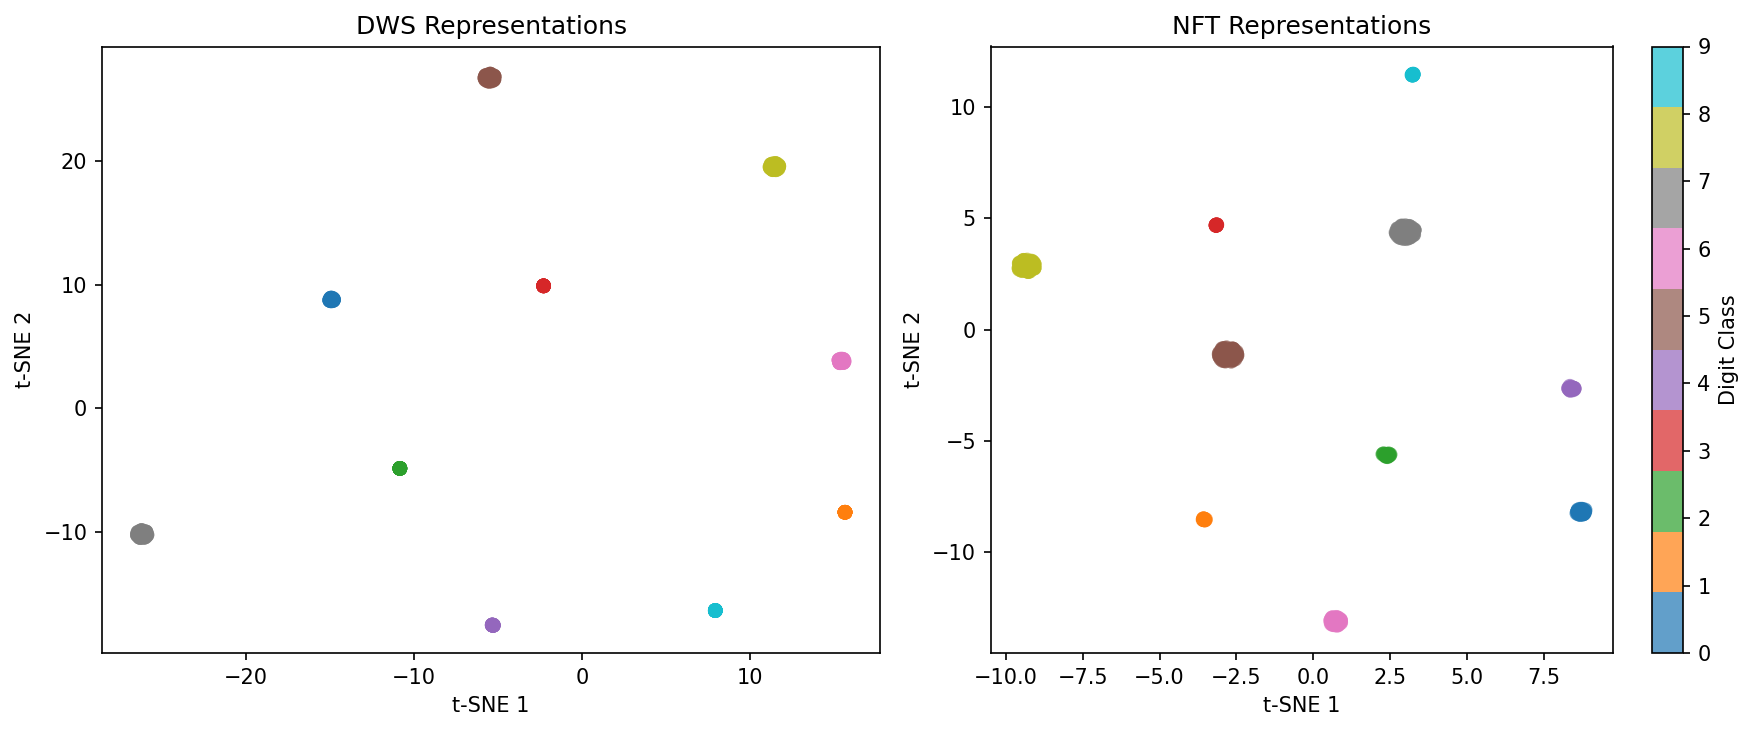
\includegraphics[width=0.9\columnwidth]{figures/tsne_representations.png}
    \caption{t-SNE visualization of weight-space representations learned by MLP, DWS, and NFT.}
    \label{fig:tsne}
\end{figure}

\begin{figure}[t]
    \centering
    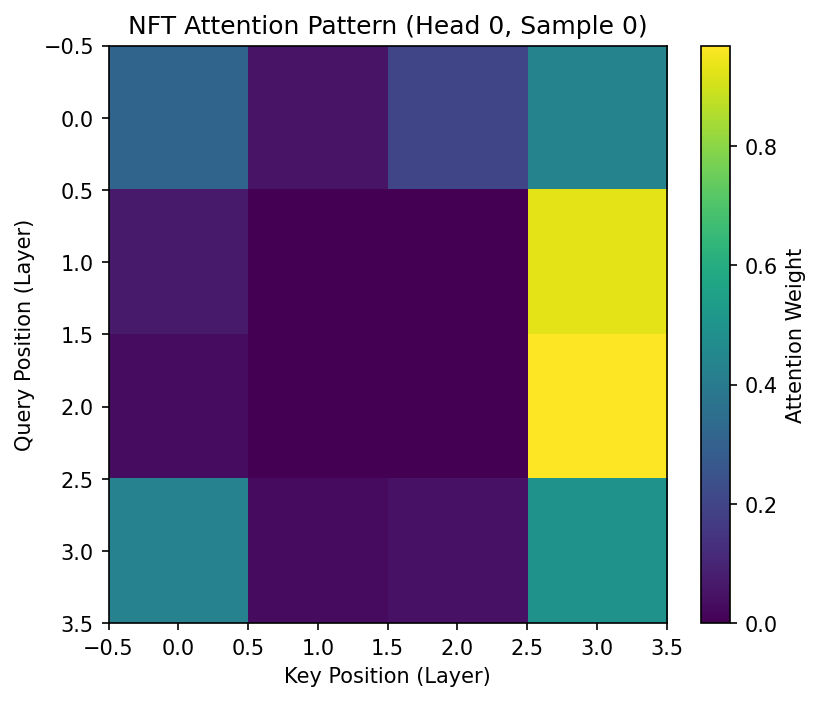
\includegraphics[width=0.9\columnwidth]{figures/attention_heatmap.png}
    \caption{NFT attention heatmap showing global information flow across weight tokens.}
    \label{fig:attention}
\end{figure}
